\documentclass[]{scrartcl}

\usepackage{graphicx}
\usepackage{subcaption}
\usepackage[margin=4.5em]{geometry}


\begin{document}

\begin{center}
	{\bfseries \Large Chicago Booth Full-Time Research Professional Application}
\end{center}

\section*{Answers (note yaxis graph)}

\subsection*{Question 1}
\textit{Please summarize key trends in median wealth over the last 30 years by race and education using plots
	and in writing.} \\ 

The trends in median wealth by race and education are shown in Figure \ref{fig:gen_trends}. Most apparent are the level differences in wealth between either white individuals compared to black and Hispanic individuals in the left panel or between the college educated and less educated in the right panel. In terms of trends all races have been experiencing growth in their median incomes over the last 30 years. However, while white median wealth grew by only 23\% on average between 1989 and 2016, black (Hispanic) wealth grew by 102\% (206\%). Looking at wealth by level education reveals a somewhat different picture. The college educated experienced a median wealth growth of 25\%, while individuals with some (or no) college education saw their median wealth shrink by 24\% (22\%) on average. \\
Further, one can see that groups that were already wealthy (white, college educated) experienced particularly strong growth in the build-up to the financial crisis in 2007. Nonetheless, it appears that all groups suffered strongly from the financial collapse afterwards.
\begin{figure}[h]
	\centering
	\begin{subfigure}{.49\textwidth}
		\centering
		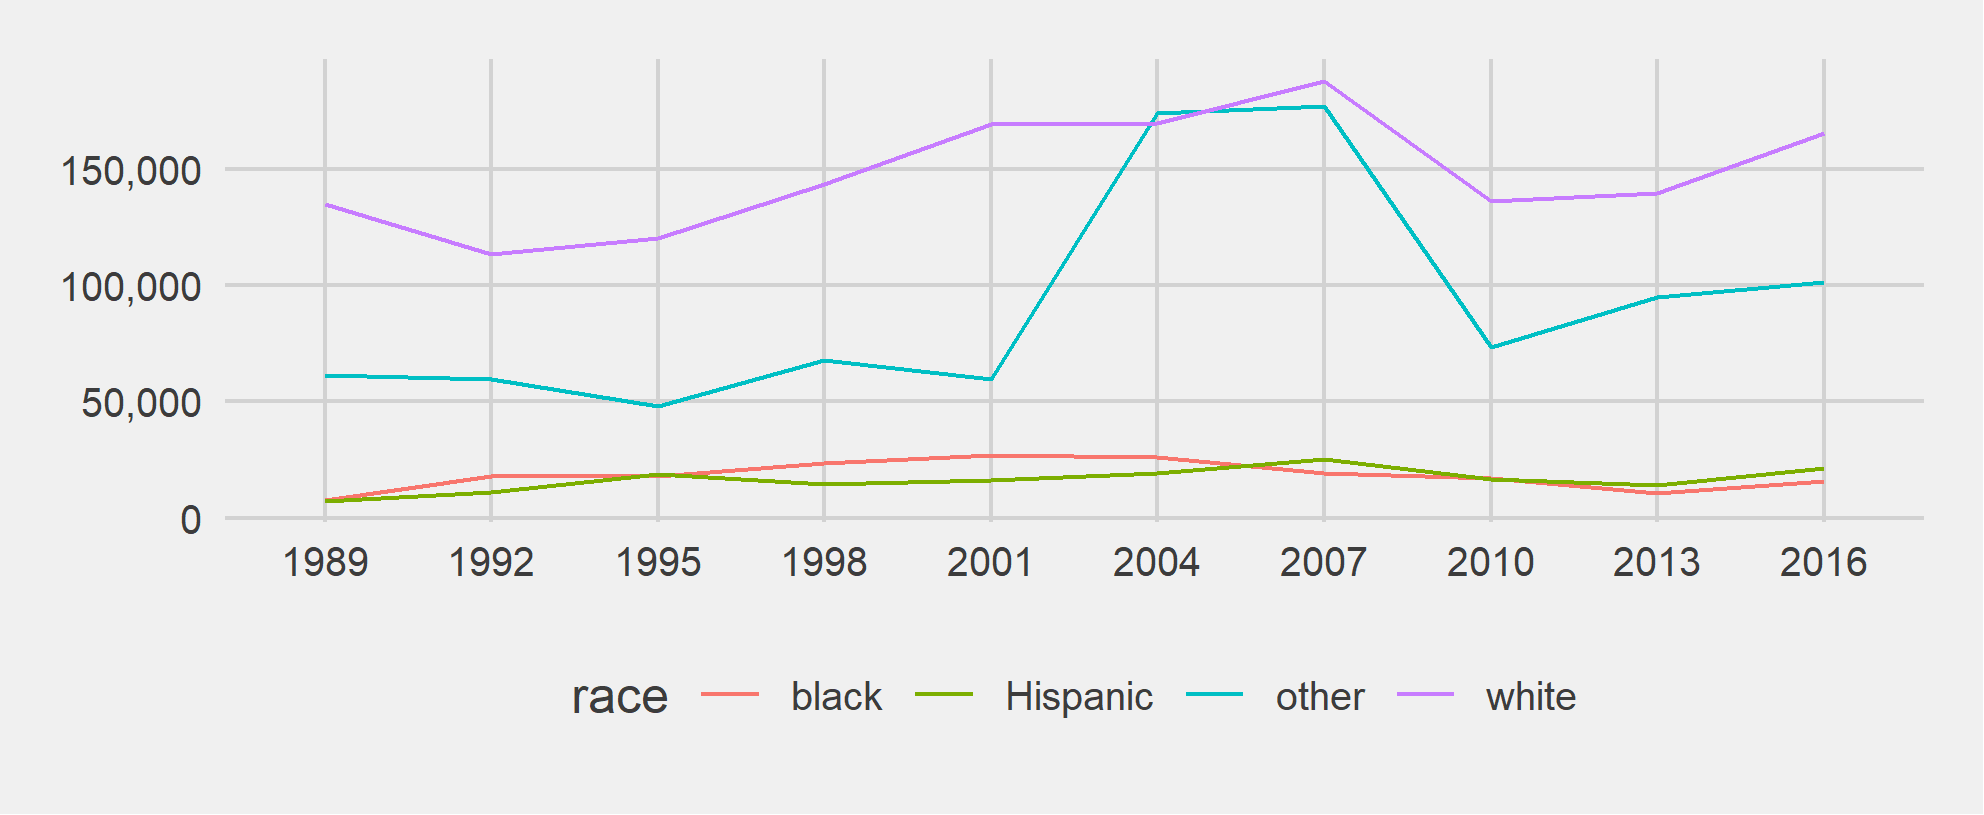
\includegraphics[width=\linewidth, height=5cm]{../median wealth finance_survey _by race .png}
	\end{subfigure}
	\begin{subfigure}{.49\textwidth}
	\centering
	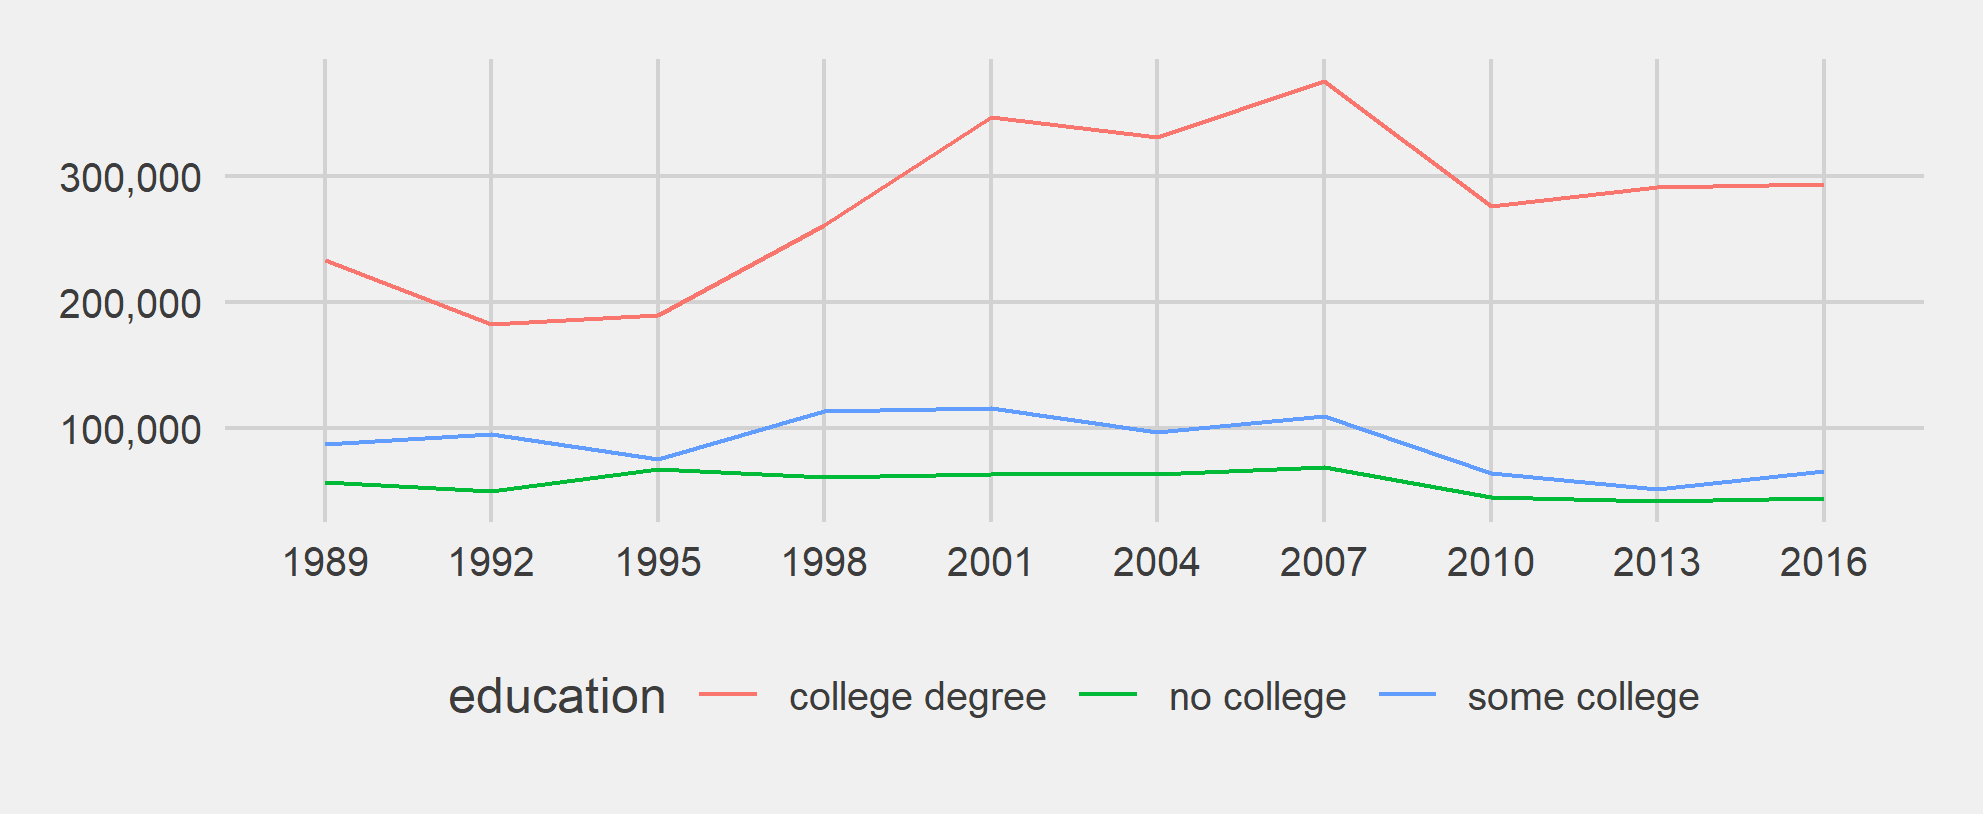
\includegraphics[width=\linewidth, height=5cm]{../median wealth finance_survey _by education .png}
	\end{subfigure}
	\begin{subfigure}{.49\textwidth}
	\centering
	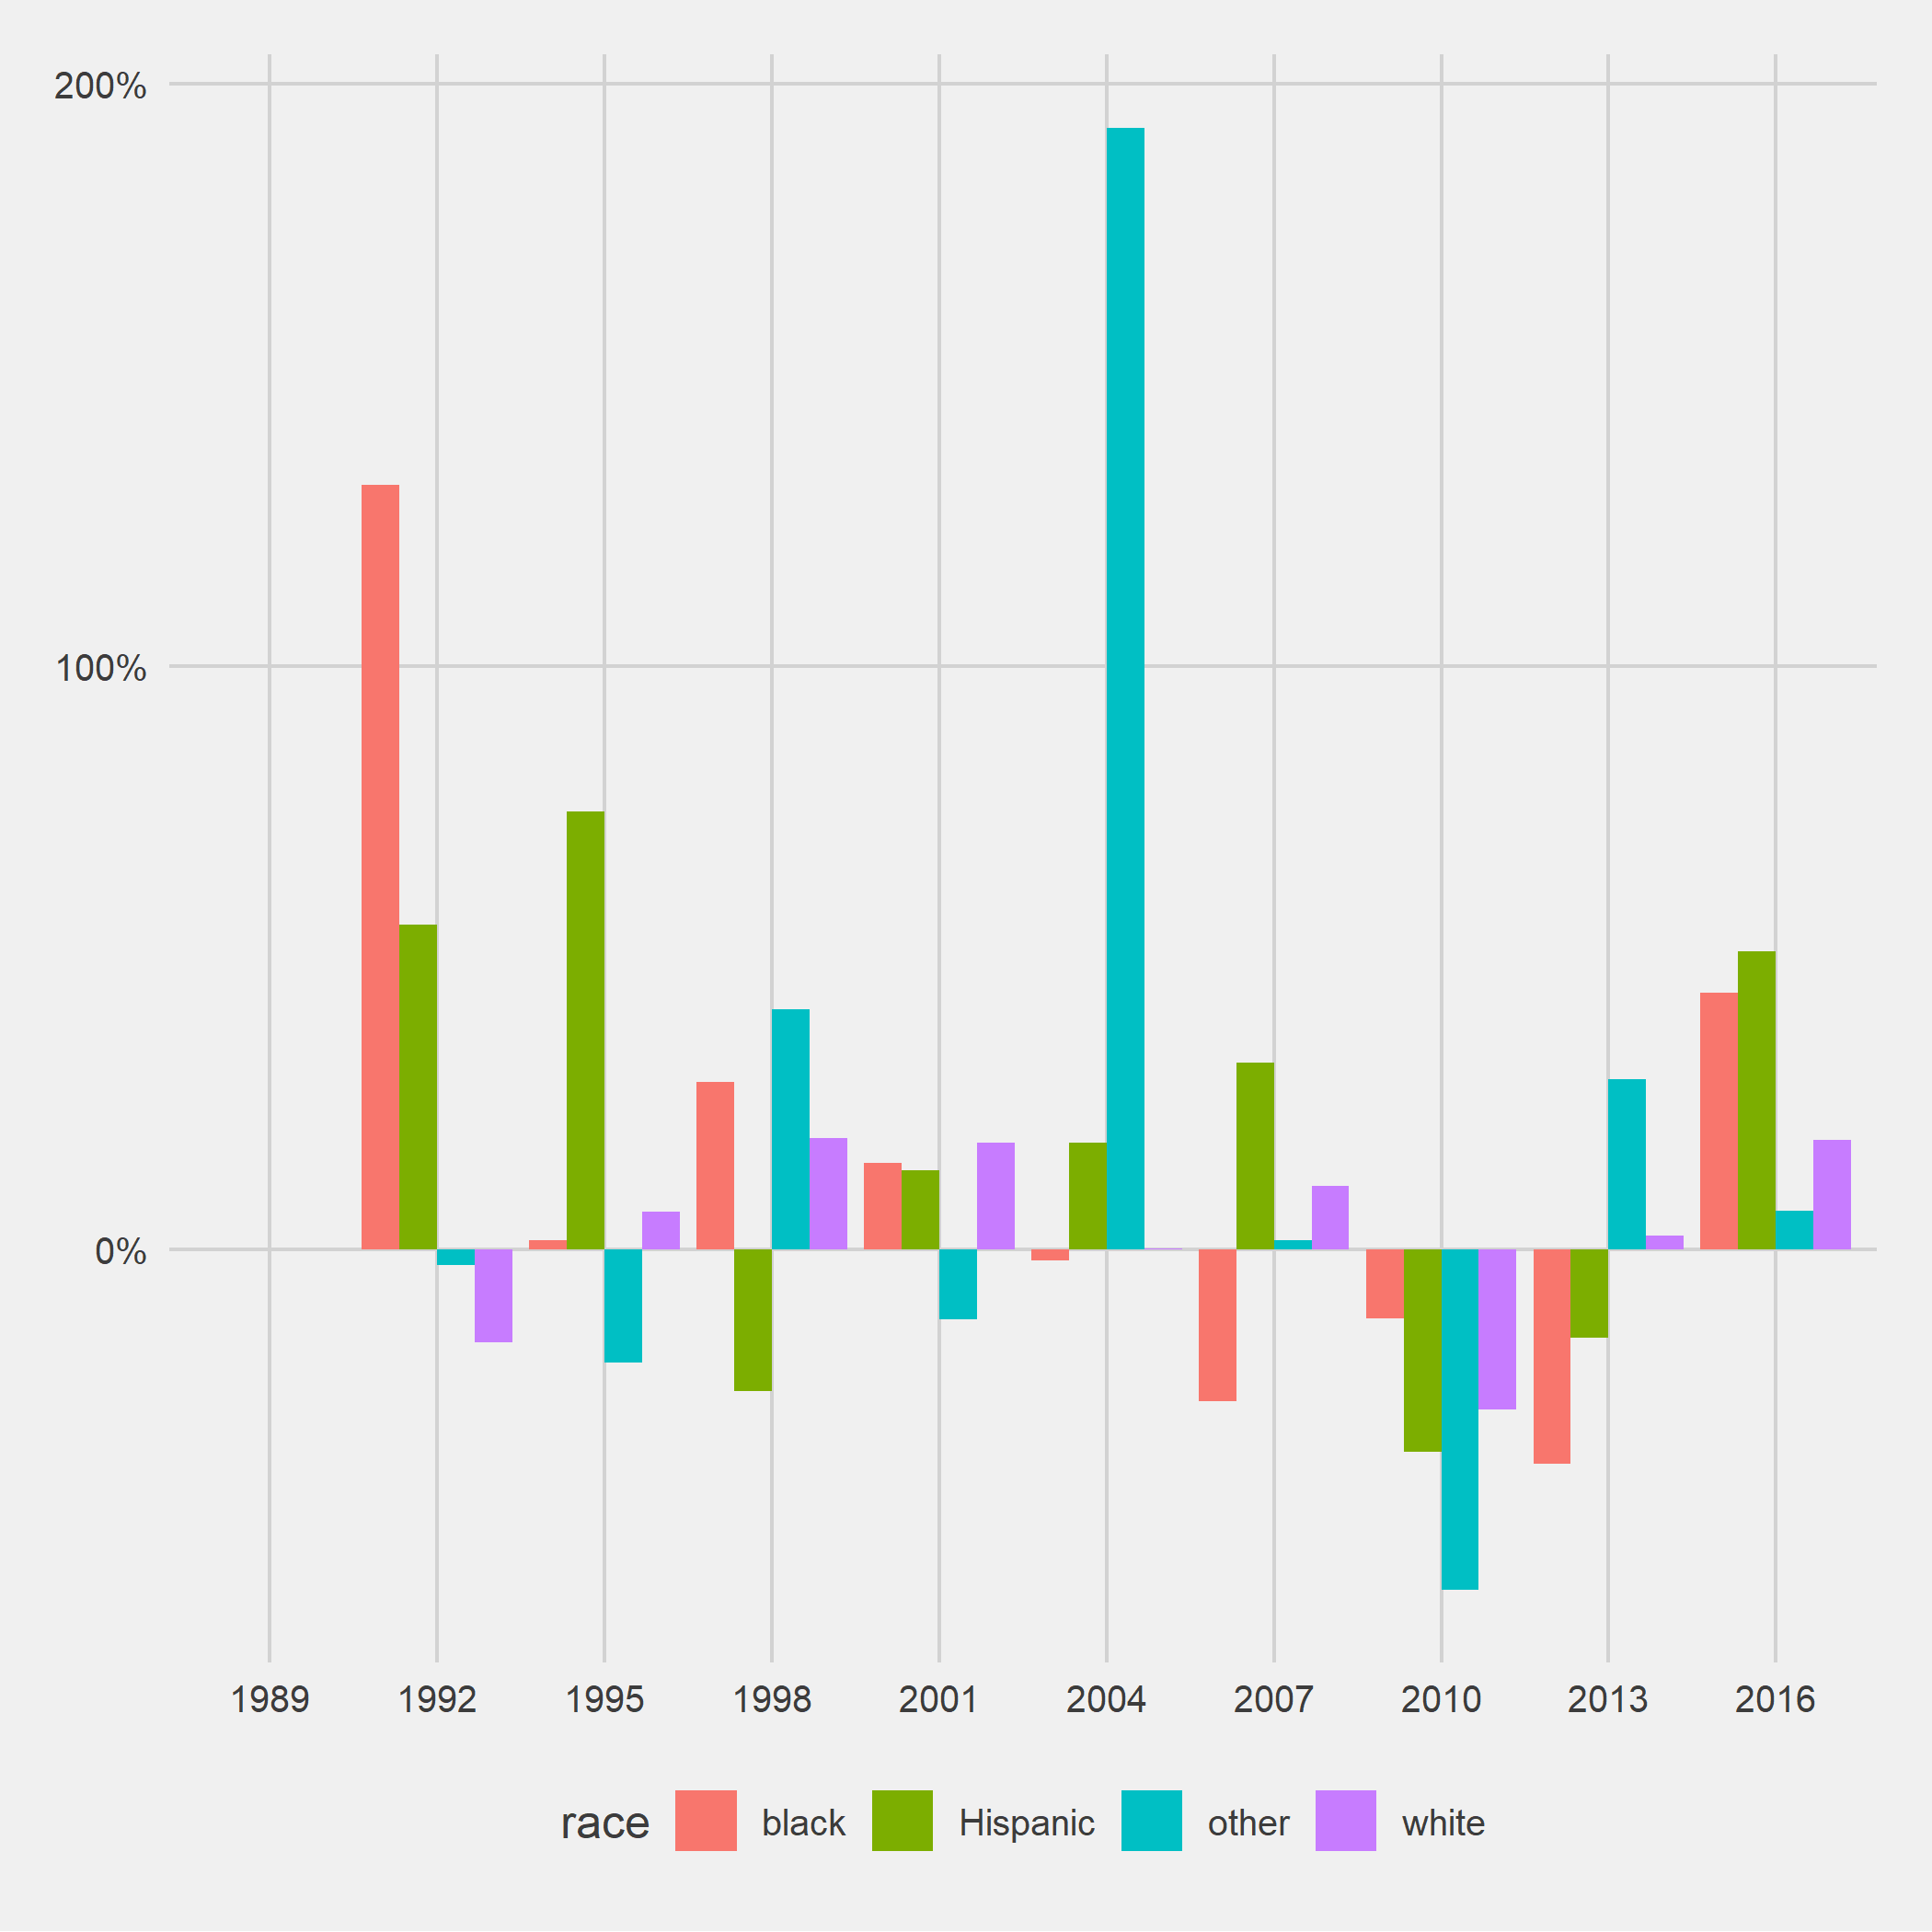
\includegraphics[width=\linewidth, height=6.5cm]{../change_median wealth finance_survey _by race .png}
	\end{subfigure}
	\begin{subfigure}{.49\textwidth}
	\centering
	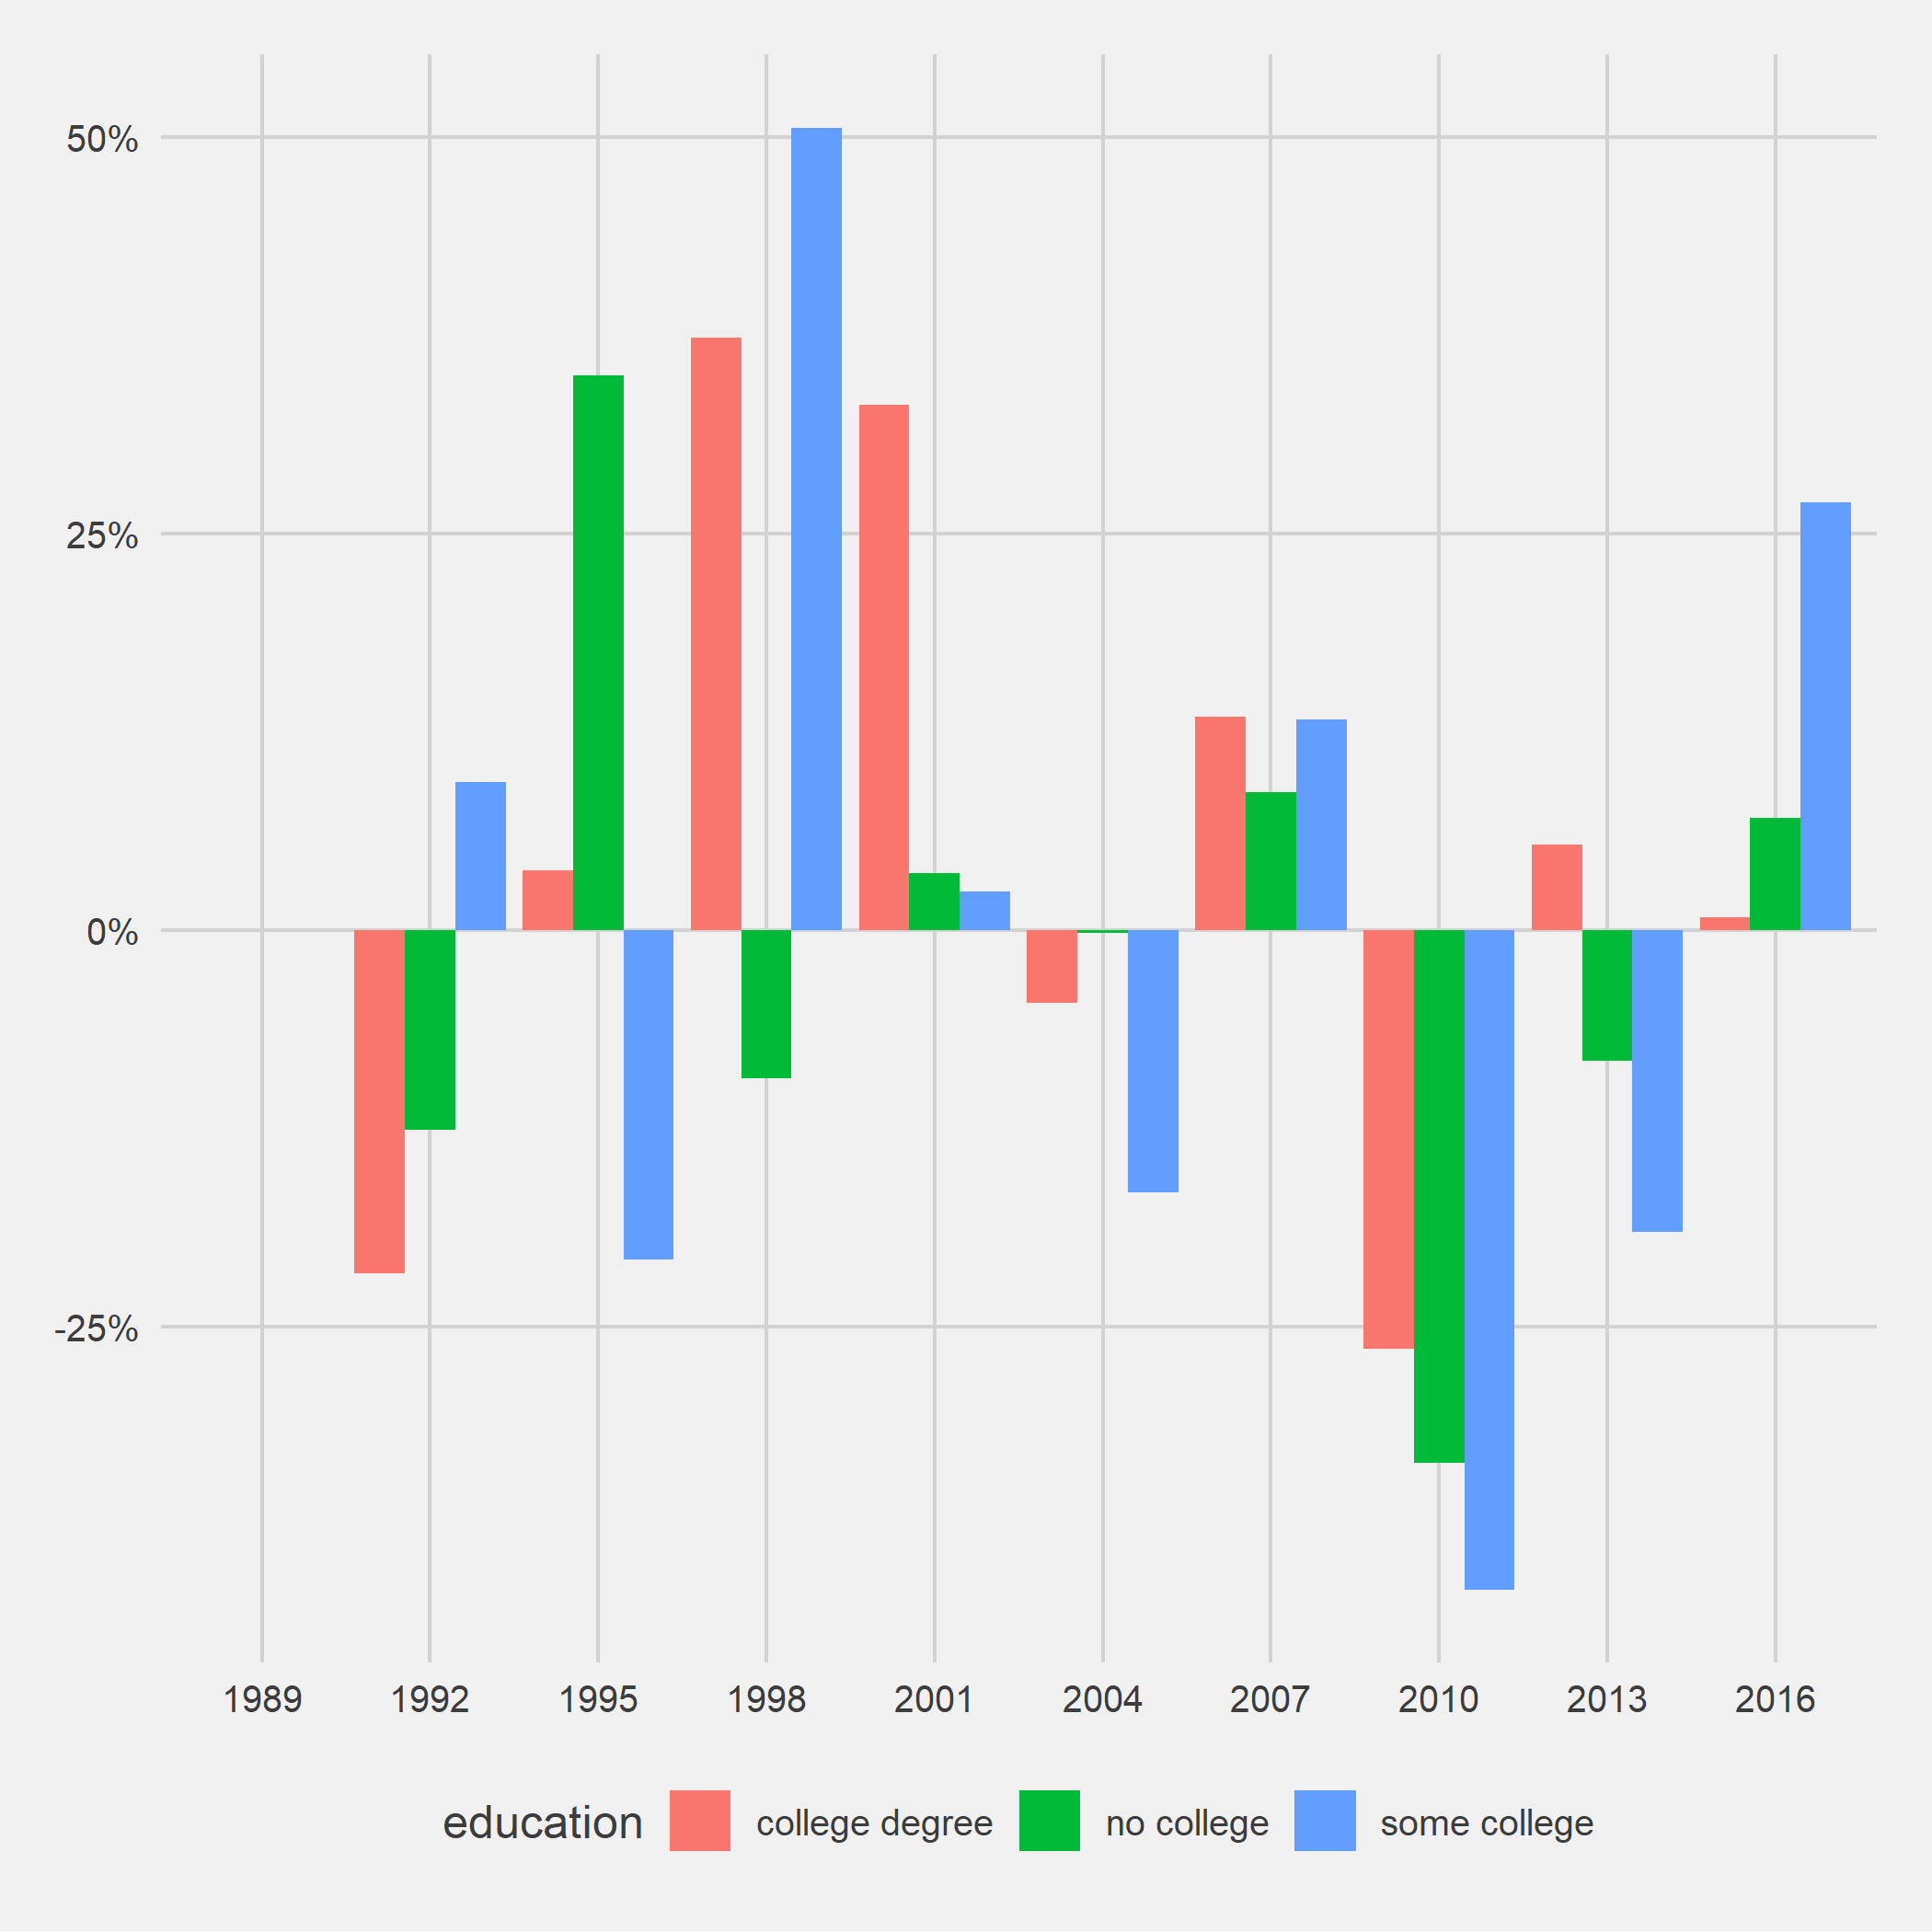
\includegraphics[width=\linewidth, height=6.5cm]{../change_median wealth finance_survey _by education .png}
	\end{subfigure}
	\caption{Median wealth in 2016 \$ over time by race and level of education}\label{fig:gen_trends}
\end{figure}

\subsection*{Question 2}
\textit{Repeat your analysis for just housing wealth for black and white households.} \\
\begin{table}[h]
	\centering
	\caption{Housing Wealth Losses per Race}
	\label{key}
	\begin{tabular}{@{\extracolsep{5pt}} lcc|cc}
		\\[-1.8ex]\hline
		\hline \\[-1.8ex]
		& \multicolumn{2}{c}{Median} & \multicolumn{2}{c}{Mean} \\ \hline
		&	Loss	&	Percentage Loss &	Loss	&	Percentage Loss \\ \hline
		\bfseries{Three Years after 2007} & & \\
		Black	&	-6,238\$	& -100\% & -20,013\$ & -30\% \\
		White	&	-31,548\$& -36\% & -43,839\$ & -23\% \\
		\bfseries{Nine Years after 2007} & & \\
		Black	&	-6,238\$ & -100\% & -20,377\$ & -30\% \\
		White	&	-18,851\$ & -21\% & -28,702\$ & -15\% \\
		\hline \\[-1.8ex]
	\end{tabular}
\end{table}

\end{document}
